% !TEX program = xelatex
% !TEX options = -shell-escape -synctex=1 -interaction=nonstopmode -file-line-error "%DOC%"
% =====================================================================
%  Seminar Ansible Configuration Management — slide Beamer
%  Theme: beamerthemeFIT.sty
%  Biên dịch:  make        (hoặc: tectonic ansible-seminar.tex)
% =====================================================================
\documentclass[aspectratio=169,11pt,xcolor=table]{beamer}
\usetheme{FIT}

% ----------------------- THÔNG TIN NHÓM (sửa tại đây) ----------------
\newcommand{\fitgroup}{Nhóm 9}
\newcommand{\fitids}{24120184 - 24120294 - 24120288 - 24120468 - 24120276}
\newcommand{\fitlecturer}{Lê Hà Minh}
\newcommand{\fitmembers}{Lê Quốc Hưng, Nguyễn Đức Duy, Nguyễn Thành Dự, Âu Bảo Trân, Mai Thúc Hải Đăng}
\title{ANSIBLE CONFIGURATION MANAGEMENT}
\subtitle{Seminar — Đề tài 9}

% Tiêu đề các phần (hiện trên slide mục lục, theo đúng thứ tự \section)
\newcommand{\fitagendaitems}{%
  {Bài toán \& sự ra đời},{Kiến trúc Agentless},
  {Các thành phần cơ bản},{Idempotence},
  {Module chuyên dụng vs Shell},{Ansible Vault}}

% Logo công cụ trong bảng: \toollogo[chiều cao tối đa]{tên file sau "logo-"}
\newcommand{\toollogo}[2][0.5cm]{\raisebox{0pt}[\dimexpr\height+3pt\relax][3pt]{\includegraphics[width=2.3cm,height=#1,keepaspectratio]{images/logo-#2.png}}}

\begin{document}

% =====================================================================
\fittitleframe
% =====================================================================

% =====================================================================
\section{Bài toán \& sự ra đời}
% =====================================================================

\begin{frame}{Bài toán: từ 1 server lên 50 server}
  \centering
  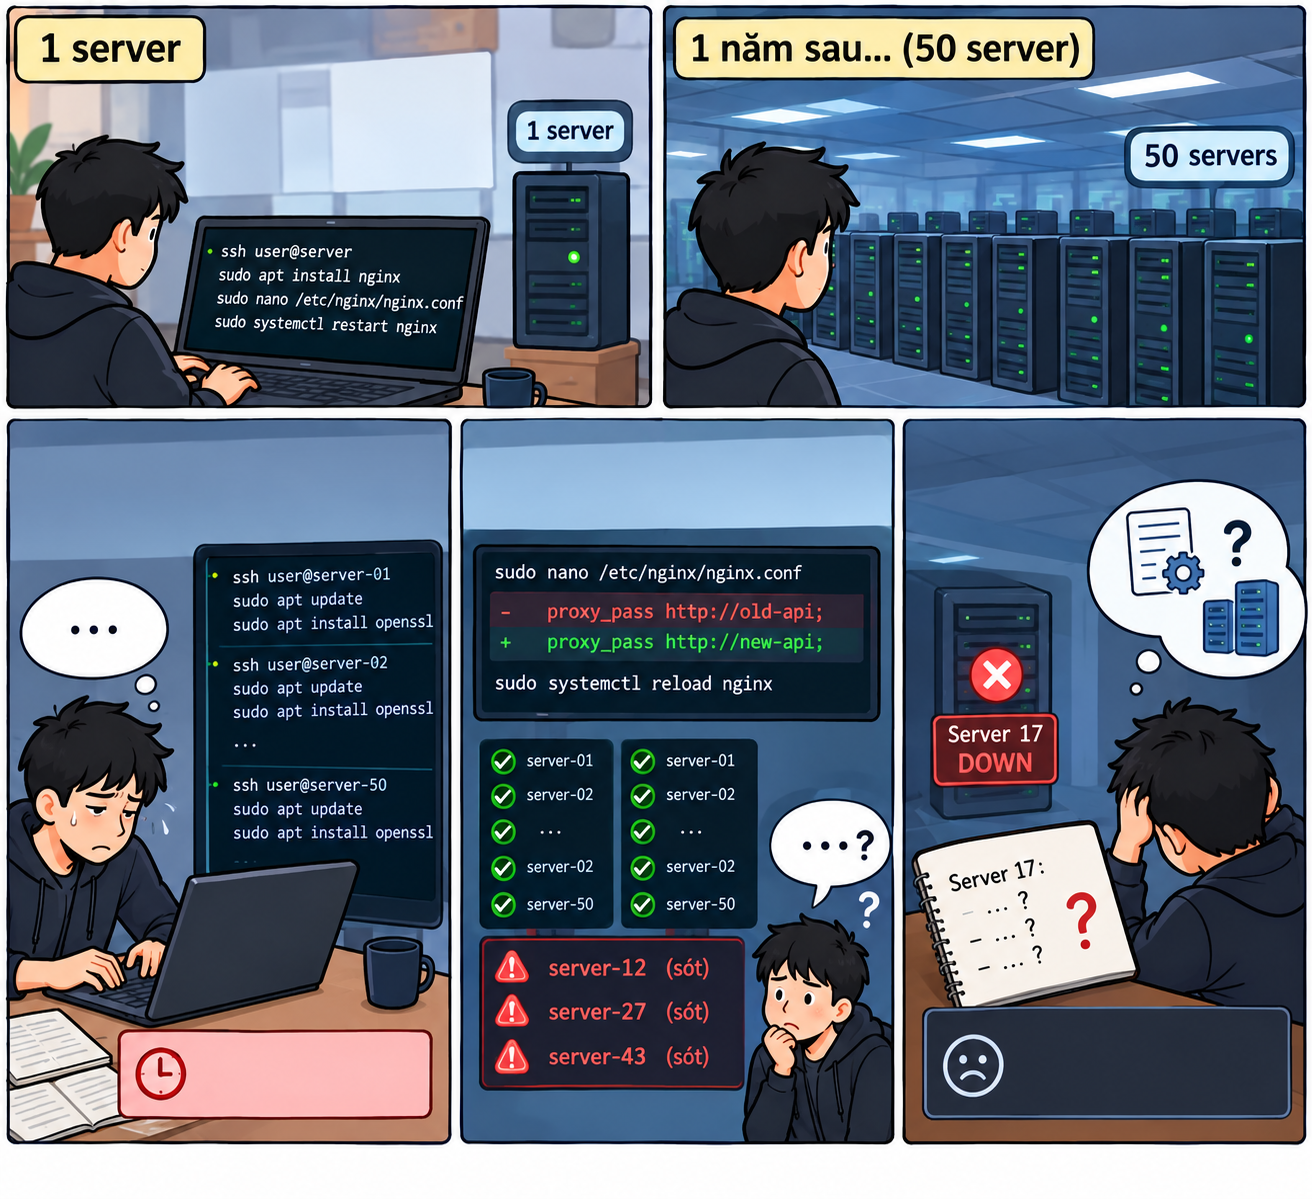
\includegraphics[width=\textwidth,height=0.84\textheight,keepaspectratio]{images/baitoan.png}
\end{frame}

\begin{frame}{Thử giải bằng tay và bằng script bash}
  \begin{fittable}{>{\bfseries}p{3.1cm} Y Y}
    & \hd{Làm tay} & \hd{Script bash} \\
    Nhiều máy & Rất tốn công, dễ sót & Tự viết vòng lặp, tự xử lý lỗi \\
    Chạy lại & Gõ lại từ đầu & Lỗi ở bước đã làm rồi
      (\code{mkdir: File exists}, \code{useradd: already exists}) \\
    Biết máy đang ra sao & Không & Không \\
    Tài liệu hoá & Nằm trong đầu người làm & Script dài, khó đọc \\
  \end{fittable}
  \vspace{0.4cm}
  \begin{fitnote}
    \textbf{Hậu quả — Configuration drift:} mỗi máy lệch đi một kiểu sau nhiều lần sửa tay.
  \end{fitnote}
\end{frame}

\begin{frame}{Hướng giải: Configuration Management \& IaC}
  \begin{itemize}\setlength{\itemsep}{0.4cm}
    \item Không viết \emph{``làm thế nào''} mà \textbf{mô tả trạng thái mong muốn}:
          \emph{``nginx phải được cài, config phải có nội dung X, service phải đang chạy''}.
    \item Công cụ tự so sánh với hiện trạng và \textbf{chỉ sửa phần lệch}
          $\rightarrow$ chạy lại bao nhiêu lần cũng an toàn (\textbf{idempotent}).
    \item \textbf{Infrastructure as Code}: cấu hình là file code
          $\rightarrow$ lưu Git, review, dựng lại server từ file.
  \end{itemize}
  \vspace{0.3cm}
  \centering
  \begin{tikzpicture}[box/.style={rounded corners=3pt, fill=fitBlue, text=white,
      minimum height=0.75cm, text width=3.2cm, align=center, font=\small\bfseries},
      ar/.style={-{Stealth[length=2.5mm]}, thick, fitBlue}]
    \node[box] (a) {Trạng thái mong muốn\\(file code)};
    \node[box, right=1cm of a] (b) {So sánh\\với hiện trạng};
    \node[box, right=1cm of b] (c) {Chỉ sửa\\phần lệch};
    \draw[ar] (a) -- (b); \draw[ar] (b) -- (c);
  \end{tikzpicture}
\end{frame}

\begin{frame}{Thế hệ công cụ đầu tiên}
  \begin{fittable}{>{\centering\arraybackslash}m{2.6cm} >{\centering\arraybackslash}m{1cm} Y Y Y}
    \hd{Công cụ} & \hd{Năm} & \hd{Agent} & \hd{Mô hình} & \hd{Ngôn ngữ} \\[2pt]
    \toollogo{cfengine} & 1993 & Có agent & Pull & DSL riêng \\[2pt]
    \toollogo{puppet} & 2005 & Có agent & Pull & Puppet DSL \\[2pt]
    \toollogo[0.8cm]{chef} & 2009 & Có agent (Chef Infra Client) & Pull & Ruby DSL \\[2pt]
    \toollogo[0.35cm]{salt} & 2011 & \code{salt-minion} (Salt SSH thì agentless) & Push / lịch chạy & YAML + Jinja2 \\[2pt]
  \end{fittable}
  \vspace{0.35cm}
  Giải quyết được bài toán, nhưng phải:
  \begin{itemize}
    \item Cài và cập nhật \textbf{agent trên từng máy}, dựng \textbf{server trung tâm},
          quản lý \textbf{chứng chỉ/key}.
    \item Học \textbf{DSL hoặc Ruby} trước khi viết được cấu hình đầu tiên.
  \end{itemize}
\end{frame}

\begin{frame}{Ansible ra đời (2012)}
  \centering
  
\includegraphics[width=\textwidth,height=0.84\textheight,keepaspectratio]{images/Ansible-radoi.png}
\end{frame}

% =====================================================================
\section{Kiến trúc Agentless}
% =====================================================================

\begin{frame}{Agentless là gì?}
  \begin{itemize}\setlength{\itemsep}{0.4cm}
    \item \textbf{Agent} = chương trình chạy thường trực trên mỗi máy được quản lý, liên lạc với
          server trung tâm để nhận cấu hình (Puppet agent, Chef Infra Client, salt-minion).
    \item \textbf{Agentless} = không cài agent riêng của Ansible trên máy đích. Ansible chỉ cài trên
          \textbf{Control Node}, khi cần thì kết nối tới \textbf{Managed Node} qua kênh có sẵn
          (\textbf{SSH} với Linux, WinRM/SSH với Windows), làm xong thì rút ra.
  \end{itemize}
  \vspace{0.5cm}
  \begin{fitnote}
    Ansible \textbf{chủ động đẩy} (push) cấu hình khi được ra lệnh, thay vì mỗi máy
    phải cài agent và tự kéo (pull) định kỳ.
  \end{fitnote}
\end{frame}

\begin{frame}{Agent vs Agentless}
  \centering
  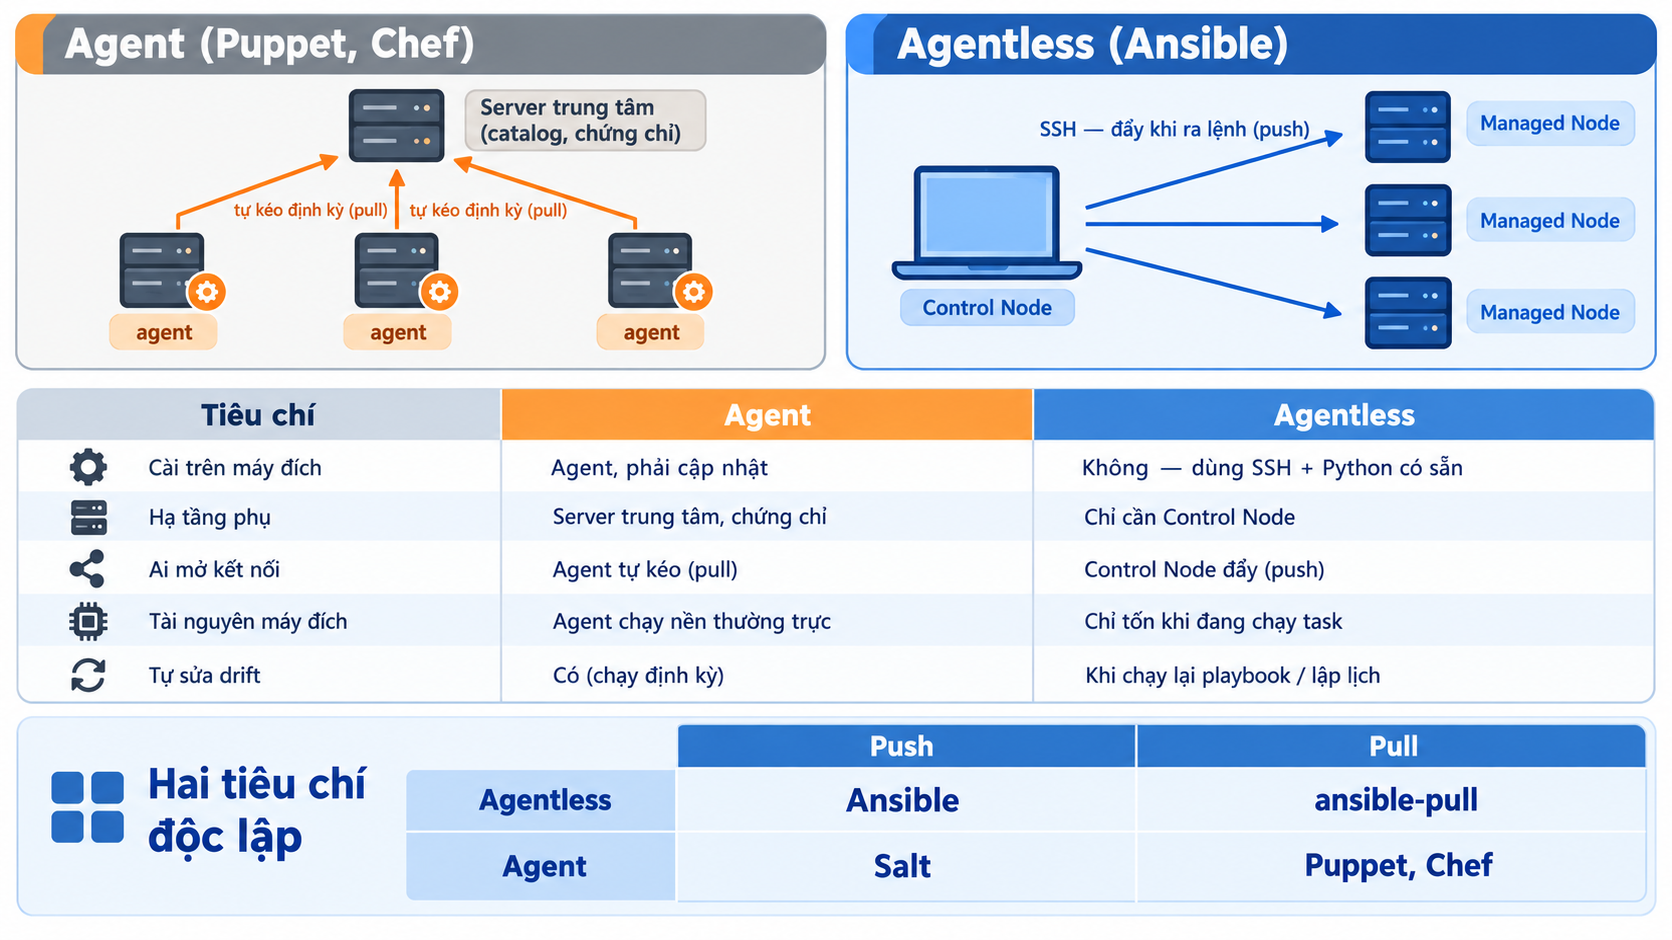
\includegraphics[width=\textwidth,height=0.84\textheight,keepaspectratio]{images/SoSanh.png}
\end{frame}

\begin{frame}{Yêu cầu của Control Node và Managed Node}
  \begin{fittable}{>{\bfseries}p{1.8cm} Y Y}
    & \hd{Control Node} & \hd{Managed Node (Linux)} \\
    Ansible & Cài \code{ansible} / \code{ansible-core} & Không cần \\
    Python & Phiên bản được bản Ansible hỗ trợ
           & Cần cho phần lớn module (không bắt buộc cùng phiên bản với Control Node) \\
    SSH & SSH client & SSH server đang chạy, mở cổng TCP 22 \\
    Khác & Inventory, playbook, private key
         & Tài khoản có shell; quyền \code{sudo} nếu task cần root \\
  \end{fittable}
  \vspace{0.3cm}
  \begin{itemize}
    \item Control Node phải là \textbf{Linux/macOS} (Windows thì dùng WSL);
          Managed Node có thể là Windows.
    \item Module \code{raw} chạy được cả khi máy đích chưa có Python
          $\rightarrow$ dùng để cài Python lần đầu.
    \item \code{become: true} = chạy bằng \code{sudo}; \textbf{không tự cấp quyền} sudo
          (\code{-K} để nhập mật khẩu sudo).
  \end{itemize}
\end{frame}

% =====================================================================
\section{Các thành phần cơ bản}
% =====================================================================

\begin{frame}{Bức tranh tổng thể}
  \centering\vspace{0.15cm}
  \begin{tikzpicture}[
      nd/.style={rounded corners=3pt, fill=fitBlue, text=white, font=\small\bfseries,
        minimum height=0.8cm, minimum width=2.5cm, align=center},
      tk/.style={rounded corners=3pt, draw=fitBlue, thick, fill=fitLight, font=\small,
        minimum height=0.65cm, minimum width=1.5cm},
      md/.style={rounded corners=2pt, draw=fitBlue!55, fill=white,
        font=\scriptsize\ttfamily, text=fitCode, minimum height=0.6cm,
        text width=3.2cm, align=center},
      ar/.style={-{Stealth[length=2mm]}, thick, fitBlue}]
    \node[nd] (inv) at (0,0) {Inventory};
    \node[nd] (pb) at (2.8,0) {Playbook};
    \node[nd, text width=3.2cm] (play) at (6.0,0)
      {Play\\[-2pt]{\scriptsize\mdseries nhóm máy + role cần chạy}};
    \draw[ar] (inv) -- (pb); \draw[ar] (pb) -- (play);

    \foreach \m/\y [count=\i] in {apt/-1.5, template/-2.45, service/-3.4} {
      \node[tk] (t\i) at (4.0,\y) {Task \i};
      \node[md] (m\i) at (7.2,\y) {module \m};
      \draw[ar] (t\i) -- (m\i);
      % đường nối đi dọc bên trái các Task, rồi rẽ vào mép trái Task
      \draw[thick, fitBlue] ([xshift=-1.2cm]play.south west) |- (t\i.west);
    }
    % thân dọc nối từ Play xuống
    \draw[thick, fitBlue] (play.west) -| ([xshift=-1.2cm]play.south west);

    \node[nd, fill=fitGreen] (h) at (10.5,-2.45) {Handler};
    \draw[ar, fitGreen] (m2.east) -- (h.west);
    \node[font=\scriptsize\itshape, text=fitGreen, above=0.05cm of h] {notify};

    % Role
    \begin{scope}[on background layer]
      \node[draw=fitBlue, dashed, rounded corners=5pt, fit=(t1)(m3)(h), inner sep=0.3cm] (role) {};
    \end{scope}
    \node[anchor=north, font=\small, align=center] at ([yshift=-0.1cm]role.south)
      {\textbf{Role} = đóng gói tasks / handlers / templates / vars thành thư mục chuẩn};
  \end{tikzpicture}
\end{frame}

\begin{frame}[fragile]{Inventory}
  \begin{columns}[c]
    \begin{column}{0.42\textwidth}
\begin{codeblock}{ini}
# inventory
[webservers]
node1 ansible_host=54.255.185.187

[webservers:vars]
ansible_user=ubuntu
\end{codeblock}
    \end{column}
    \begin{column}{0.54\textwidth}
      \begin{itemize}\setlength{\itemsep}{0.3cm}
        \item Inventory = \textbf{danh sách máy} Ansible quản lý, chia thành \textbf{nhóm}.
        \item Nhóm mặc định \code{all}; biến tách ra \code{group\_vars/} và \code{host\_vars/}.
        \item \textbf{Cụ thể hơn thắng}:\\
              \code{host\_vars} > \code{group\_vars/<nhóm>} > \code{group\_vars/all}.
      \end{itemize}
    \end{column}
  \end{columns}
\end{frame}

\begin{frame}[fragile]{Kết nối SSH key}
  \centering
  \begin{tikzpicture}[
      nd/.style={rounded corners=3pt, draw=fitBlue, thick, fill=fitLight, align=center,
        font=\scriptsize, minimum width=4.1cm, minimum height=0.85cm}]
    \node[nd] (c) {\textbf{Control Node}\\ansible-core, private key};
    \node[nd, right=2.6cm of c] (m) {\textbf{Managed Node} \code{<managed-ip>}\\ví dụ: 54.255.185.187};
    \draw[-{Stealth[length=2.5mm]}, very thick, fitBlue] (c) -- node[above, font=\scriptsize]
      {SSH (TCP 22)} (m);
  \end{tikzpicture}
  \par\vspace{0.15cm}
  \begin{columns}[t]
    \begin{column}{0.58\textwidth}
\begin{codeblock}[minted options={fontsize=\tiny}]{bash}
ssh-keygen -t ed25519 -f ~/.ssh/ansible_lab
ssh-copy-id -i ~/.ssh/ansible_lab.pub ubuntu@54.255.185.187
ansible webservers -i inventory -m ansible.builtin.ping
# "pong" = SSH + Python OK (không phải ICMP)
\end{codeblock}
    \end{column}
    \begin{column}{0.4\textwidth}
\begin{codeblock}[minted options={fontsize=\tiny}]{ini}
# inventory
[webservers]
node1 ansible_host=54.255.185.187

[webservers:vars]
ansible_user=ubuntu
ansible_ssh_private_key_file=~/.ssh/ansible_lab
\end{codeblock}
    \end{column}
  \end{columns}
  \raggedright
  \begin{itemize}\small
    \item Private key \textbf{không bao giờ rời control node}; public key nằm trong
          \code{authorized\_keys} của máy đích.
  \end{itemize}
\end{frame}

\begin{frame}[fragile]{Playbook \& Task}
  \begin{columns}[c]
    \begin{column}{0.4\textwidth}
\begin{codeblock}{yaml}
- name: Cài nginx
  hosts: webservers
  become: true
  tasks:
    - name: Đảm bảo nginx đã cài
      ansible.builtin.apt:
        name: nginx
        state: present
\end{codeblock}
    \end{column}
    \begin{column}{0.56\textwidth}
      \begin{itemize}\small\setlength{\itemsep}{0.2cm}
        \item \textbf{Play}: \code{hosts}, \code{become}, \code{vars},
              \code{tasks} (chạy từ trên xuống), \code{handlers}.
        \item \textbf{Task} = \code{name} + module + tham số; hay kèm
              \code{when}, \code{loop}, \code{register}, \code{notify}.
        \item \code{ansible.builtin.apt} = tên đầy đủ \textbf{(FQCN)}:
              collection \code{ansible.builtin} + module \code{apt}.
        \item \textbf{YAML}: thụt lề bằng \textbf{space}, \code{key: value},
              list dùng \mbox{\code{-}.}
        \item \textbf{Ad-hoc} (\code{ansible webservers -i inventory -m ping}): chạy \textbf{1 module, 1 lần}
              từ dòng lệnh, không cần file. \textbf{Playbook}: nhiều task, lưu Git,
              chạy lại được.
      \end{itemize}
    \end{column}
  \end{columns}
\end{frame}

\begin{frame}{Một task chạy như thế nào?}
  \begin{columns}[c]
    \begin{column}{0.56\textwidth}
      \begin{enumerate}\setlength{\itemsep}{0.25cm}
        \item Control node đọc inventory, playbook, biến $\rightarrow$ đóng gói module + tham số.
        \item SSH vào managed node, tạo thư mục tạm, chuyển mã module sang.
        \item Managed node chạy module bằng Python (dùng \code{become} nếu cần quyền root).
        \item Module trả \textbf{JSON} $\rightarrow$ Ansible báo
              \code{ok} / \code{changed} / \code{failed}.
        \item Xoá file tạm; kết quả task (gói, file cấu hình) vẫn giữ.
      \end{enumerate}
    \end{column}
    \begin{column}{0.42\textwidth}
      \centering
      \begin{tikzpicture}[
          nd/.style={rounded corners=3pt, fill=fitBlue, text=white, font=\small\bfseries,
            minimum width=2.4cm, minimum height=0.8cm, align=center},
          ar/.style={-{Stealth[length=2mm]}, thick, fitBlue},
          st/.style={circle, fill=fitBlue, text=white, font=\tiny\bfseries, inner sep=1pt,
            minimum size=1.1em}]
        \node[nd] (c) at (0,0) {Control\\Node};
        \node[nd] (m) at (0,-3.4) {Managed\\Node};
        \draw[ar] ([xshift=-0.5cm]c.south) -- node[left, font=\scriptsize, align=right]
          (l2) {module\\qua SSH} ([xshift=-0.5cm]m.north);
        \draw[ar] ([xshift=0.5cm]m.north) -- node[right, font=\scriptsize, align=left]
          (l4) {JSON\\kết quả} ([xshift=0.5cm]c.south);
        \node[st, above=0.05cm of l2] {2};
        \node[st, above=0.05cm of l4] {4};
        \node[st, left=0.15cm of c] {1};
        \node[st, left=0.15cm of m] {3};
        \node[st, right=0.15cm of m] {5};
      \end{tikzpicture}
    \end{column}
  \end{columns}
\end{frame}

\begin{frame}[fragile]{Role}
  \begin{columns}[c]
    \begin{column}{0.56\textwidth}
\begin{codeblock}[minted options={fontsize=\scriptsize}]{text}
roles/nginx/
├── defaults/main.yml       # biến mặc định
├── handlers/main.yml       # handler restart Nginx
├── tasks/main.yml          # các task triển khai
├── templates/nginx.conf.j2 # template cấu hình
└── vars/vault.yml          # secret đã mã hoá
\end{codeblock}
    \end{column}
    \begin{column}{0.4\textwidth}
      \begin{itemize}\setlength{\itemsep}{0.35cm}
        \item Role \textbf{không tự chạy}; \code{site.yml} gọi bằng \code{roles: [nginx]}.
        \item File Vault được nạp qua \code{vars\_files} trước khi role chạy.
        \item Ưu tiên biến:\\
              \code{defaults} < \code{group\_vars} < \code{host\_vars}
              < \code{vars} (role) < \code{-e}\\
              (extra vars \textbf{luôn thắng}).
      \end{itemize}
    \end{column}
  \end{columns}
\end{frame}

\begin{frame}[fragile]{Template Jinja2}
  \begin{columns}[t]
    \begin{column}{0.5\textwidth}
      \begin{itemize}\small
        \item \code{\{\{ biến \}\}} in giá trị · \code{\{\% if \%\}} / \code{\{\% for \%\}}
              điều khiển · \code{\{\# \#\}} comment.
        \item Filter hay dùng: \code{default(80)}, \code{join(' ')}.
        \item Render \textbf{trên control node} rồi mới đẩy file sang máy đích.
      \end{itemize}
      \vspace{0.2cm}
      \begin{fittable}{>{\bfseries}l Y Y}
        & \hd{\code{\color{white}copy}} & \hd{\code{\color{white}template}} \\
        Nội dung & Nguyên văn & Render biến rồi đẩy \\
        Dùng cho & File tĩnh & File đổi theo host/môi trường \\
      \end{fittable}
    \end{column}
    \begin{column}{0.46\textwidth}
\begin{codeblock}[minted options={fontsize=\scriptsize}]{jinja}
server {
    listen {{ http_port }} default_server;
    server_name {{ server_name }};
    root {{ document_root }};
    location / {
        try_files $uri $uri/ =404;
    }
}
\end{codeblock}
    \end{column}
  \end{columns}
\end{frame}

\begin{frame}[fragile]{Handler}
  \begin{columns}[t]
    \begin{column}{0.5\textwidth}
      \begin{itemize}\setlength{\itemsep}{0.25cm}
        \item Chỉ chạy khi task \code{notify} báo \textbf{\code{changed}} — config không đổi
              thì không restart.
        \item Chạy \textbf{cuối play}, \textbf{1 lần mỗi host} dù được notify nhiều lần.
        \item Tên trong \code{notify} phải \textbf{khớp} tên handler.
      \end{itemize}
      \vspace{0.2cm}
      \begin{fitnote}
        Đề yêu cầu \emph{restart}; thực tế nên dùng \code{state: reloaded}
        (không downtime) khi chỉ đổi config.
      \end{fitnote}
    \end{column}
    \begin{column}{0.46\textwidth}
\begin{codeblock}[minted options={fontsize=\scriptsize}]{yaml}
- name: Render nginx.conf
  ansible.builtin.template:
    src: nginx.conf.j2
    dest: >-
      /etc/nginx/sites-available/default
  notify: Restart Nginx

# handlers/main.yml
- name: Restart Nginx
  ansible.builtin.service:
    name: nginx
    state: restarted
\end{codeblock}
    \end{column}
  \end{columns}
\end{frame}

% =====================================================================
\section{Idempotence}
% =====================================================================

\begin{frame}{Idempotent là gì?}
  \begin{itemize}\setlength{\itemsep}{0.3cm}
    \item \textbf{Idempotent} (tính luỹ đẳng): một thao tác áp dụng \textbf{nhiều lần}
          cho \textbf{cùng kết quả} như áp dụng \textbf{một lần}.
    \item Trong Ansible: chạy playbook \textbf{1 lần hay 100 lần} $\rightarrow$ máy luôn ở
          \textbf{cùng trạng thái mong muốn}, không tác dụng phụ.
          Lần đầu sửa những gì còn lệch (\code{changed}), các lần sau chỉ báo \code{ok}.
    \item Ví dụ đời thường: bấm \textbf{nút tầng 5} thang máy nhiều lần vẫn chỉ đi tầng 5;
          còn \textbf{công tắc đèn} bấm 2 lần thì về lại trạng thái cũ $\rightarrow$ không idempotent.
  \end{itemize}
  \vspace{0.3cm}
  \centering
  \begin{tikzpicture}[
      run/.style={rounded corners=3pt, draw=fitBlue, thick, fill=fitLight, align=center,
        font=\scriptsize, minimum width=2.6cm, minimum height=0.85cm},
      ar/.style={-{Stealth[length=2mm]}, thick, fitBlue}]
    \node[run] (r1) {\textbf{Lần 1}\\\code{changed=3}};
    \node[run, right=1cm of r1] (r2) {\textbf{Lần 2}\\\code{changed=0}};
    \node[run, right=1cm of r2] (rn) {\textbf{Lần N}\\\code{changed=0}};
    \draw[ar] (r1) -- (r2); \draw[ar] (r2) -- (rn);
  \end{tikzpicture}
  \par\vspace{0.3cm}
  \begin{fitnote}
    Vì sao là \textbf{cốt lõi}: chạy lại playbook luôn \textbf{an toàn} — sửa được máy bị lệch cấu hình,
    chạy tiếp sau khi lỗi giữa chừng, không lo cài trùng hay ghi đè sai.
  \end{fitnote}
\end{frame}

\begin{frame}{Khai báo vs Mệnh lệnh}
  \begin{columns}[c]
    \begin{column}{0.48\textwidth}
      \begin{itemize}\setlength{\itemsep}{0.35cm}
        \item Shell script: \emph{``làm thế nào''}.\\
              Ansible: \emph{``kết quả cuối là gì''}.
        \item Module: \textbf{kiểm tra hiện trạng} $\rightarrow$ khớp thì \code{ok},
              lệch thì sửa vừa đủ $\rightarrow$ \code{changed}.
      \end{itemize}
    \end{column}
    \begin{column}{0.48\textwidth}
      \begin{fittable}{>{\ttfamily\color{fitCode}}l Y}
        \hd{PLAY RECAP} & \hd{Ý nghĩa} \\
        ok & Thành công (bao gồm cả \code{changed}) \\
        changed & Đã thay đổi máy đích \\
        failed & Lỗi, dừng play trên host đó \\
        unreachable & Không SSH được tới host \\
        skipped & \code{when} trả về false \\
      \end{fittable}
    \end{column}
  \end{columns}
\end{frame}

\begin{frame}{Xem trước: \texttt{-{}-check} \& \texttt{-{}-diff}}
  \begin{itemize}\setlength{\itemsep}{0.4cm}
    \item \code{-{}-check}: \textbf{mô phỏng}, không đổi gì trên máy đích.
    \item \code{-{}-diff}: hiện \textbf{dòng thêm/bớt} trong file.
    \item Giới hạn: \code{shell}/\code{command} bị \textbf{skip} trong check mode
          (trừ khi có \code{creates}/\code{removes}).
  \end{itemize}
  \vspace{0.4cm}
  \begin{fitnote}
    \code{ansible-playbook site.yml -{}-check -{}-diff} — xem trước thay đổi trước khi áp dụng thật.
  \end{fitnote}
\end{frame}

% =====================================================================
\section{Module chuyên dụng vs Shell}
% =====================================================================

\begin{frame}{\texttt{command} vs \texttt{shell}}
  \begin{fittable}{>{\bfseries}p{4.2cm} Y Y}
    & \hd{\code{\color{white}command}} & \hd{\code{\color{white}shell}} \\
    Chạy qua \code{/bin/sh} & Không & Có \\
    Pipe, redirect, \code{\$VAR} & Không & Có \\
    Rủi ro shell injection & \textcolor{fitGreen}{\textbf{Thấp}} & \textcolor{fitRed}{\textbf{Cao}} \\
  \end{fittable}
  \vspace{0.4cm}
  \begin{itemize}\setlength{\itemsep}{0.25cm}
    \item \textbf{Bẫy}: \code{command: echo data >> /tmp/x} $\rightarrow$ \textbf{không tạo file}
          (\code{>>} thành đối số) nhưng vẫn báo \code{changed}.
    \item \code{raw} (không cần Python, dùng bootstrap) và \code{script} (chạy script có sẵn)
          chỉ dùng trường hợp đặc biệt.
  \end{itemize}
\end{frame}

\begin{frame}{Vì sao module chuyên dụng tốt hơn?}
  \begin{itemize}\setlength{\itemsep}{0.2cm}
    \item \code{shell}/\code{command} là \textbf{``hộp đen''}: Ansible chỉ thấy \code{rc},
          \code{stdout} $\rightarrow$ \textbf{luôn báo \code{changed}}.
    \item Module chuyên dụng \textbf{kiểm tra trước khi làm}:
      \begin{itemize}
        \item \code{copy}: so checksum, giống thì \code{ok}.
        \item \code{lineinfile}: dòng đã có thì \code{ok}, chưa có thì thêm.
        \item \code{systemd\_service}: \code{state: started} chỉ khởi động khi đang dừng.
      \end{itemize}
    \item Kèm theo: hỗ trợ \code{-{}-check}/\code{-{}-diff}, trả dữ liệu có cấu trúc,
          an toàn hơn, dễ đọc.
  \end{itemize}
\end{frame}

\begin{frame}[fragile]{Khi buộc phải dùng shell}
  \vspace{0.3cm}
\begin{codeblock}{yaml}
- ansible.builtin.shell: tar -xzf app.tar.gz -C /opt/app
  args:
    creates: /opt/app/README     # đã có file này thì bỏ qua

- ansible.builtin.command: uname -r
  changed_when: false            # lệnh chỉ đọc
\end{codeblock}
  \vspace{0.4cm}
  \begin{itemize}\setlength{\itemsep}{0.25cm}
    \item \code{creates} / \code{removes}: cho Ansible biết khi nào lệnh \textbf{đã làm rồi}
          $\rightarrow$ bỏ qua, giữ idempotent.
    \item \code{changed\_when: false}: lệnh chỉ đọc thì \textbf{không báo \code{changed}}.
  \end{itemize}
\end{frame}

% =====================================================================
\section{Ansible Vault}
% =====================================================================

\begin{frame}{Vault là gì?}
  \begin{itemize}\setlength{\itemsep}{0.35cm}
    \item Secret để \textbf{plain text} trong Git sẽ \textbf{lộ vĩnh viễn} (Git nhớ lịch sử).
    \item Vault mã hoá \textbf{AES256} $\rightarrow$ secret vẫn nằm trong Git nhưng đã mã hoá.
    \item Lệnh: \code{create}, \code{encrypt}, \code{view}, \code{edit}, \code{decrypt}, \code{rekey};
          \code{encrypt\_string} mã hoá \textbf{từng giá trị} (tên biến vẫn đọc được).
    \item Chạy: \code{-{}-ask-vault-pass} (chạy tay) hoặc \code{-{}-vault-password-file}
          (tự động; file \code{chmod 600} + \code{.gitignore}).
  \end{itemize}
\end{frame}

\begin{frame}[fragile]{Cách tổ chức}
  \vspace{0.3cm}
\begin{codeblock}{text}
group_vars/web/
├── vars.yml    # công khai:  app_secret: "{{ vault_app_secret }}"
└── vault.yml   # ĐÃ MÃ HOÁ:  vault_app_secret: "..."
\end{codeblock}
  \vspace{0.4cm}
  \begin{itemize}\setlength{\itemsep}{0.3cm}
    \item Tiền tố \code{vault\_} $\rightarrow$ grep được tên biến, biết ngay giá trị thật
          nằm trong vault.
    \item Task dùng secret thêm \code{no\_log: true} để \textbf{không in secret} ra màn hình.
  \end{itemize}
\end{frame}

\begin{frame}{Hạn chế của Ansible}
  \begin{itemize}\setlength{\itemsep}{0.3cm}
    \item \textbf{Chậm khi nhiều máy}: mỗi task phải SSH vào và đẩy module sang;
          mặc định chỉ chạy song song \code{forks = 5} máy.
    \item \textbf{Không tự sửa khi lệch cấu hình}: không có agent nên ai sửa tay trên máy
          thì Ansible không biết $\rightarrow$ phải chạy lại playbook (hoặc lên lịch chạy định kỳ).
    \item \textbf{Playbook lớn khó đọc}: YAML + Jinja2 + \code{when}/\code{loop} dễ rối,
          debug khó hơn code thông thường.
    \item \textbf{Không quản lý vòng đời hạ tầng}: không lưu state như Terraform
          $\rightarrow$ không hợp để tạo/xoá VM hàng loạt.
  \end{itemize}
\end{frame}

\begin{frame}[fragile]{Ví dụ 1: Terraform dựng máy, Ansible cấu hình}
  \centering
  \begin{tikzpicture}[
      st/.style={rounded corners=3pt, draw=fitBlue, thick, fill=fitLight, align=center,
        font=\scriptsize, minimum width=2.4cm, minimum height=0.85cm},
      ar/.style={-{Stealth[length=2mm]}, thick, fitBlue}]
    \node[st] (a) {\code{terraform apply}};
    \node[st, right=0.45cm of a] (b) {3 máy EC2\\+ IP public};
    \node[st, right=0.45cm of b] (c) {File \code{inventory}\\(Terraform tự sinh)};
    \node[st, right=0.45cm of c] (d) {\code{ansible-playbook}};
    \node[st, right=0.45cm of d, fill=fitBlue, text=white] (e) {\textbf{3 web Nginx}\\\textbf{chạy}};
    \draw[ar] (a) -- (b); \draw[ar] (b) -- (c); \draw[ar] (c) -- (d); \draw[ar] (d) -- (e);
  \end{tikzpicture}
  \par\vspace{0.2cm}
  \begin{columns}[t]
    \begin{column}{0.6\textwidth}
\begin{codeblock}[minted options={fontsize=\tiny}]{text}
# main.tf
resource "aws_instance" "web" {
  count         = 3
  ami           = "ami-xxxx"      # Ubuntu
  instance_type = "t3.micro"
}
resource "local_file" "inventory" {
  filename = "inventory"
  content  = join("\n", concat(["[webservers]"],
               aws_instance.web[*].public_ip))
}
\end{codeblock}
\begin{codeblock}[minted options={fontsize=\tiny}]{bash}
terraform apply -auto-approve
ansible-playbook -i inventory site.yml
\end{codeblock}
    \end{column}
    \begin{column}{0.38\textwidth}
      \raggedright
      \begin{itemize}\small\setlength{\itemsep}{0.25cm}
        \item Terraform lo \textbf{``có máy''}: tạo VM, mạng, security group; nhớ state để
              sửa/xoá.
        \item Ansible lo \textbf{``máy chạy đúng''}: cài gói, render config, bật service.
        \item Không ai ghi IP bằng tay; cần 10 máy thì sửa \code{count = 10}.
      \end{itemize}
    \end{column}
  \end{columns}
\end{frame}

\begin{frame}[fragile]{Ví dụ 2: CI/CD — push code là chạy playbook}
  \centering
  \begin{tikzpicture}[
      st/.style={rounded corners=3pt, draw=fitBlue, thick, fill=fitLight, align=center,
        font=\scriptsize, minimum width=2.4cm, minimum height=0.85cm},
      ar/.style={-{Stealth[length=2mm]}, thick, fitBlue}]
    \node[st] (a) {\code{git push main}};
    \node[st, right=0.45cm of a] (b) {GitHub Actions\\khởi động runner};
    \node[st, right=0.45cm of b] (c) {\code{ansible-lint}\\kiểm tra};
    \node[st, right=0.45cm of c] (d) {\code{ansible-playbook}};
    \node[st, right=0.45cm of d, fill=fitBlue, text=white] (e) {\textbf{Server}\\\textbf{được cập nhật}};
    \draw[ar] (a) -- (b); \draw[ar] (b) -- (c); \draw[ar] (c) -- (d); \draw[ar] (d) -- (e);
  \end{tikzpicture}
  \par\vspace{0.2cm}
  \begin{columns}[t]
    \begin{column}{0.6\textwidth}
\begin{codeblock}[minted options={fontsize=\tiny}]{yaml}
# .github/workflows/deploy.yml
on:
  push:
    branches: [main]
jobs:
  deploy:
    runs-on: ubuntu-latest
    env:
      ANSIBLE_HOST_KEY_CHECKING: "False"
    steps:
      - uses: actions/checkout@v4
      - run: pip install ansible ansible-lint
      - run: ansible-lint site.yml
      - run: |
          echo "${{ secrets.SSH_KEY }}" > key && chmod 600 key
          echo "${{ secrets.VAULT_PASS }}" > .vault_pass
          ansible-playbook -i inventory site.yml \
            --private-key key --vault-password-file .vault_pass
\end{codeblock}
    \end{column}
    \begin{column}{0.38\textwidth}
      \raggedright
      \begin{itemize}\small\setlength{\itemsep}{0.25cm}
        \item Private key và mật khẩu Vault cất trong \textbf{GitHub Secrets},
              không nằm trong repo.
        \item \code{ansible-lint} lỗi $\rightarrow$ pipeline dừng, không đụng tới server.
        \item Nhờ \textbf{idempotent}: push 10 lần thì chỉ phần thay đổi mới báo
              \code{changed}.
      \end{itemize}
    \end{column}
  \end{columns}
\end{frame}

\begin{frame}{Mindmap kiến thức Ansible}
  \centering
  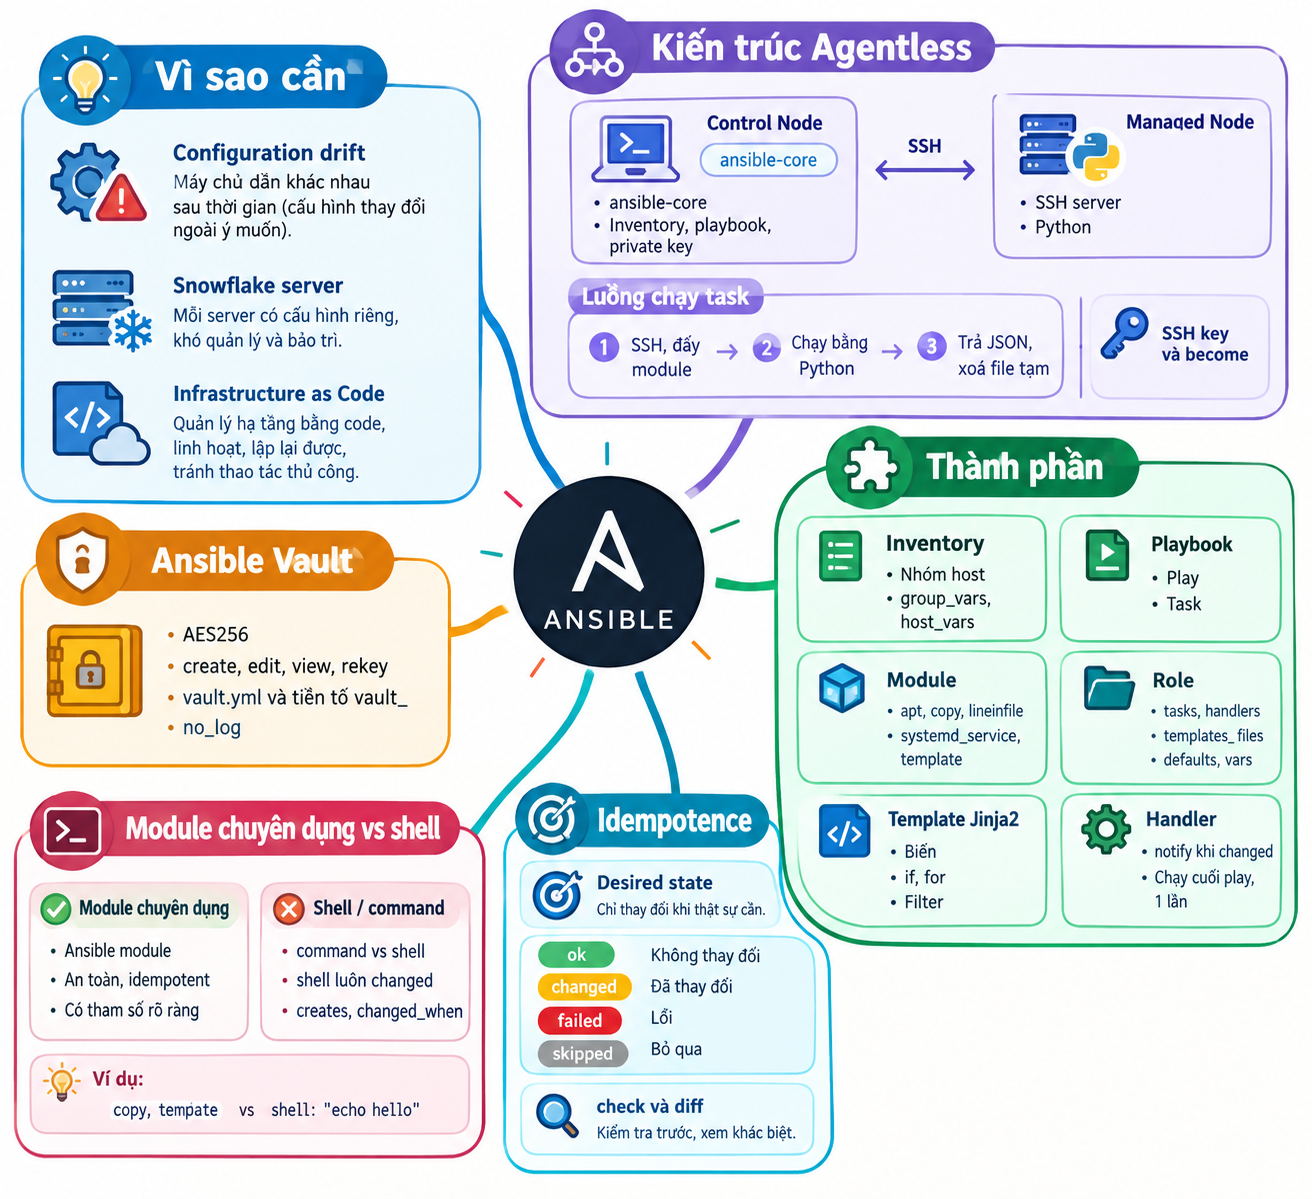
\includegraphics[width=\textwidth,height=0.84\textheight,keepaspectratio]{images/mindmap-ansible.png}
\end{frame}

\fitthanksframe{Cảm ơn thầy và các bạn đã lắng nghe!}

\end{document}
